\documentclass[10pt,a4paper]{article}
\usepackage[UTF8,fontset = windows]{ctex}
\setCJKmainfont[BoldFont=黑体,ItalicFont=楷体]{华文中宋}
\usepackage{amssymb,amsmath,amsfonts,amsthm,mathrsfs,dsfont,graphicx}
\usepackage{ifthen,indentfirst,enumerate,color,titletoc}
\usepackage{tikz}
\usepackage{multicol}
\usepackage{makecell}
\usepackage{longtable}
\usepackage{diagbox}
\usetikzlibrary{arrows,calc,intersections,patterns,decorations.pathreplacing,3d,angles,quotes,positioning}
\usepackage[bf,small,indentafter,pagestyles]{titlesec}
\usepackage[top=1in, bottom=1in,left=0.8in,right=0.8in]{geometry}
\renewcommand{\baselinestretch}{1.65}
\newtheorem{defi}{定义~}
\newtheorem{eg}{例~}
\newtheorem{ex}{~}
\newtheorem{rem}{注~}
\newtheorem{thm}{定理~}
\newtheorem{coro}{推论~}
\newtheorem{axiom}{公理~}
\newtheorem{prop}{性质~}
\newcommand{\blank}[1]{\underline{\hbox to #1pt{}}}
\newcommand{\bracket}[1]{(\hbox to #1pt{})}
\newcommand{\onech}[4]{\par\begin{tabular}{p{.9\textwidth}}
A.~#1\\
B.~#2\\
C.~#3\\
D.~#4
\end{tabular}}
\newcommand{\twoch}[4]{\par\begin{tabular}{p{.46\textwidth}p{.46\textwidth}}
A.~#1& B.~#2\\
C.~#3& D.~#4
\end{tabular}}
\newcommand{\vartwoch}[4]{\par\begin{tabular}{p{.46\textwidth}p{.46\textwidth}}
(1)~#1& (2)~#2\\
(3)~#3& (4)~#4
\end{tabular}}
\newcommand{\fourch}[4]{\par\begin{tabular}{p{.23\textwidth}p{.23\textwidth}p{.23\textwidth}p{.23\textwidth}}
A.~#1 &B.~#2& C.~#3& D.~#4
\end{tabular}}
\newcommand{\varfourch}[4]{\par\begin{tabular}{p{.23\textwidth}p{.23\textwidth}p{.23\textwidth}p{.23\textwidth}}
(1)~#1 &(2)~#2& (3)~#3& (4)~#4
\end{tabular}}
\begin{document}

\begin{center}
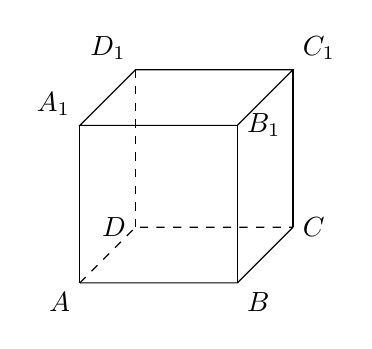
\begin{tikzpicture}[>=latex, x={(0:1)}, z={(225:0.5)}]
\def\l{2}
\draw (0,0,0) node [below left] {$A$} coordinate (A);
\draw (A) ++ (\l,0,0) node [below right] {$B$} coordinate (B);
\draw (A) ++ (\l,0,-\l) node [right] {$C$} coordinate (C);
\draw (A) ++ (0,0,-\l) node [left] {$D$} coordinate (D);
\draw (A) -- (B) -- (C);
\draw [dashed] (A) -- (D) -- (C);
\draw (A) ++ (0,\l,0) node [above left] {$A_1$} coordinate (A1);
\draw (B) ++ (0,\l,0) node [right] {$B_1$} coordinate (B1);
\draw (C) ++ (0,\l,0) node [above right] {$C_1$} coordinate (C1);
\draw (D) ++ (0,\l,0) node [above left] {$D_1$} coordinate (D1);
\draw (A1) -- (B1) -- (C1) -- (D1) -- cycle;
\draw (A) -- (A1) (B) -- (B1) (C) -- (C1);
\draw [dashed] (D) -- (D1);
\end{tikzpicture}
\end{center}

\begin{center}
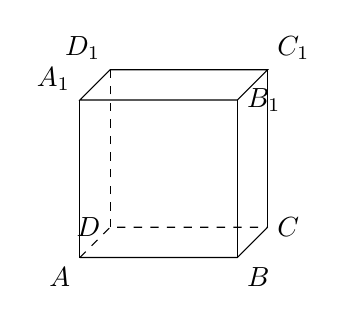
\begin{tikzpicture}[>=latex]
\def\l{2}
\def\m{1}
\def\n{2}
\draw (0,0,0) node [below left] {$A$} coordinate (A);
\draw (A) ++ (\l,0,0) node [below right] {$B$} coordinate (B);
\draw (A) ++ (\l,0,-\m) node [right] {$C$} coordinate (C);
\draw (A) ++ (0,0,-\m) node [left] {$D$} coordinate (D);
\draw (A) -- (B) -- (C);
\draw [dashed] (A) -- (D) -- (C);
\draw (A) ++ (0,\n,0) node [above left] {$A_1$} coordinate (A1);
\draw (B) ++ (0,\n,0) node [right] {$B_1$} coordinate (B1);
\draw (C) ++ (0,\n,0) node [above right] {$C_1$} coordinate (C1);
\draw (D) ++ (0,\n,0) node [above left] {$D_1$} coordinate (D1);
\draw (A1) -- (B1) -- (C1) -- (D1) -- cycle;
\draw (A) -- (A1) (B) -- (B1) (C) -- (C1);
\draw [dashed] (D) -- (D1);

\end{tikzpicture}
\end{center}


\end{document}